\documentclass[11pt]{article}
\title{Adversarial Autoencoders, Foundations of Computer Vision, Final Report}
\author{Soumyakanti Das}

\usepackage[a4paper, margin=1in]{geometry}
\usepackage{fancyhdr}
\usepackage{indentfirst}
\usepackage{float}
\usepackage{graphicx}
\usepackage{caption}
\usepackage{hyperref}
\hypersetup{
colorlinks = true
}

\pagestyle{fancy}
\fancyhf{}
\fancyhead[LE,RO]{Adversarial Autoencoders}

\begin{document}
\maketitle

\section{Introduction}

In this report, I have summarized the work that I have done for my final project,
which is on Adversarial Autoencoders.

Autoencoders are a type of neural network that has two components, encoder and
decoder. Its task is to encode its input into a condensed vector, called Latent
Code. The decoder then takes this latent code as input and produces an output
which is similar to the input. Thus, it finds application in data compression,
novel image generation and dimensionality reduction.

In Adversarial Autoencoders, a Generative Adversarial Network is added to a
standard autoencoder, which trains the autoencoder to encode its inputs more
efficiently. It does this by imposing a gaussian distribution to the Latent
Code space. It should be noted that any arbitrary distribution can also be
imposed onto the code space, but since working with gaussian distribution is
much easier, I have used it in my project.

I'm using MNIST data for training the network.

\section{Architecture}

There are three components to the network, Encoder, Decoder, and Discriminator.
For the Encoder network, I have three fully connected layers with 25\% dropout
and ReLU as activation function. The input dimension is the same as the image
size, whereas output dimension is just 2.
The Decoder network is just a mirror image of the Encoder network. Its input
dimension is 2, whereas output dimension is the size of the image. For MNIST,
the size of the image tensor is 784 (28 * 28). The decoder networks last layer
is sigmoidal.
The Discriminator network takes two inputs, one from the real gaussian
distribution and the other from the output of the encoder. Its input dimension
is 2 whereas output dimension is just 1 as it outputs the probability that the
code space vector comes from the real distribution. It also has three fully
connected layers with 20\% dropouts and ReLU activation function.

\section{Training}

Since there are three networks to be trained simultaneously, the training
process is a bit complex. First, in the Reconstruction phase, the encoder
and decoder are trained simultaneously to reduce the reconstruction error. This
is done by passing the inputs to the encoder, which outputs latent code vector,
and then passing the latent code vector to the decoder network. Binary cross
entropy loss is calculated on the output of the decoder and the original inputs.
This loss is then back propagated to both, encoder and decoder.
Next, in the Regularization phase, loss for the discriminator network is calculated
on the latent code data and data from actual gaussian distribution. The loss
is then backpropagated through the discriminator network. Finally, the
generator network, which is also the encoder of the autoencoder, is trained
again by calculating loss on its output and the output of the trained discriminator.
This loss is then back propagated through the generator (encoder) network.

I have used 0.0005, 0.0001 as my Reconstruction and Regularization
learning rates respectively, and used Adam optimizer to training all three
networks.

\section{Results}

After training the networks for 100 epochs, I get the following results.

It can be seen from Figure \ref{fig:plots} that Reconstruction and Generator
losses decrease because the Encoder (Generator) and Decoder becomes more and
more efficient, while Discriminator loss increases, which suggests that it
becomes more and more difficult for the Discriminator network to tell apart
fake samples from real ones. The encoder learns how to fool the discriminator
better with each epoch.

Figure \ref{fig:results} show the generated images after training, from random
samples of the gaussian distribution. It can be seen that the decoder is able to
generate recognizable images, only from 2 numbers, which is very interesting
and shows how efficient the adversarial training is.

Since MNIST and FashionMNIST datasets have images of equal dimensions, I tried
to generate images from FashionMNIST with the same architecture. Figure
\ref{fig:fplot} shows the training losses whereas Figure \ref{fig:fashion}
show the generated images after training for 50 epochs for the same architecture.

\begin{figure}
\centering
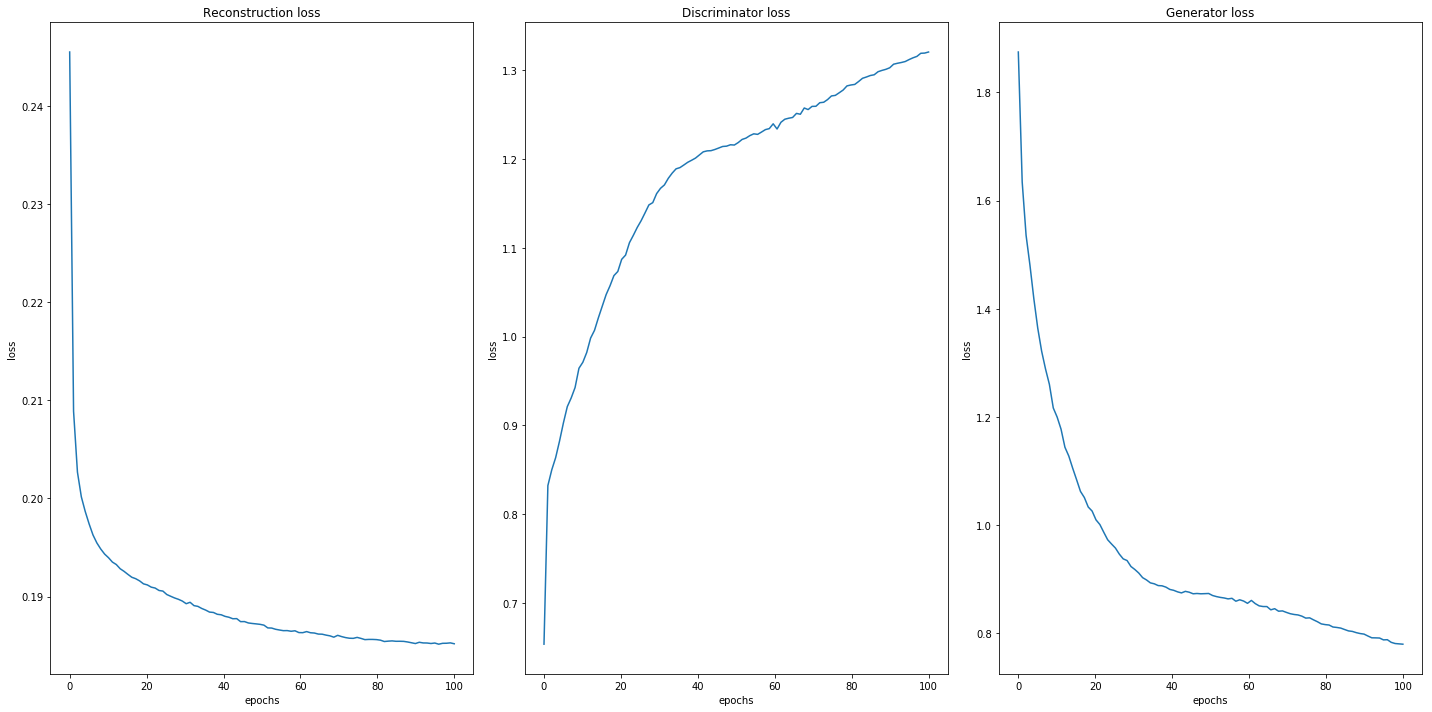
\includegraphics[width=\textwidth]{plots.png}
\caption{\label{fig:plots} Training Losses - MNIST}
\end{figure}

\begin{figure}
\centering
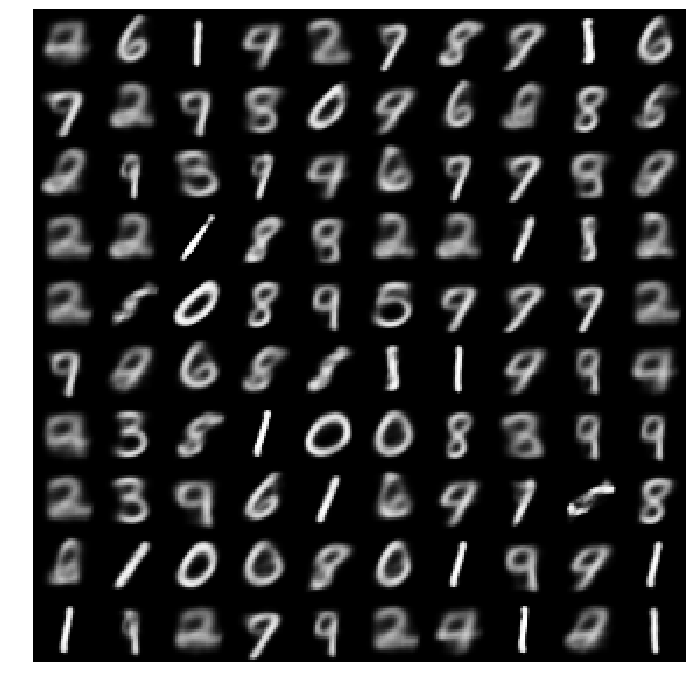
\includegraphics[width=\textwidth]{results.png}
\caption{\label{fig:results} Generated Images - MNIST}
\end{figure}

\begin{figure}
\centering
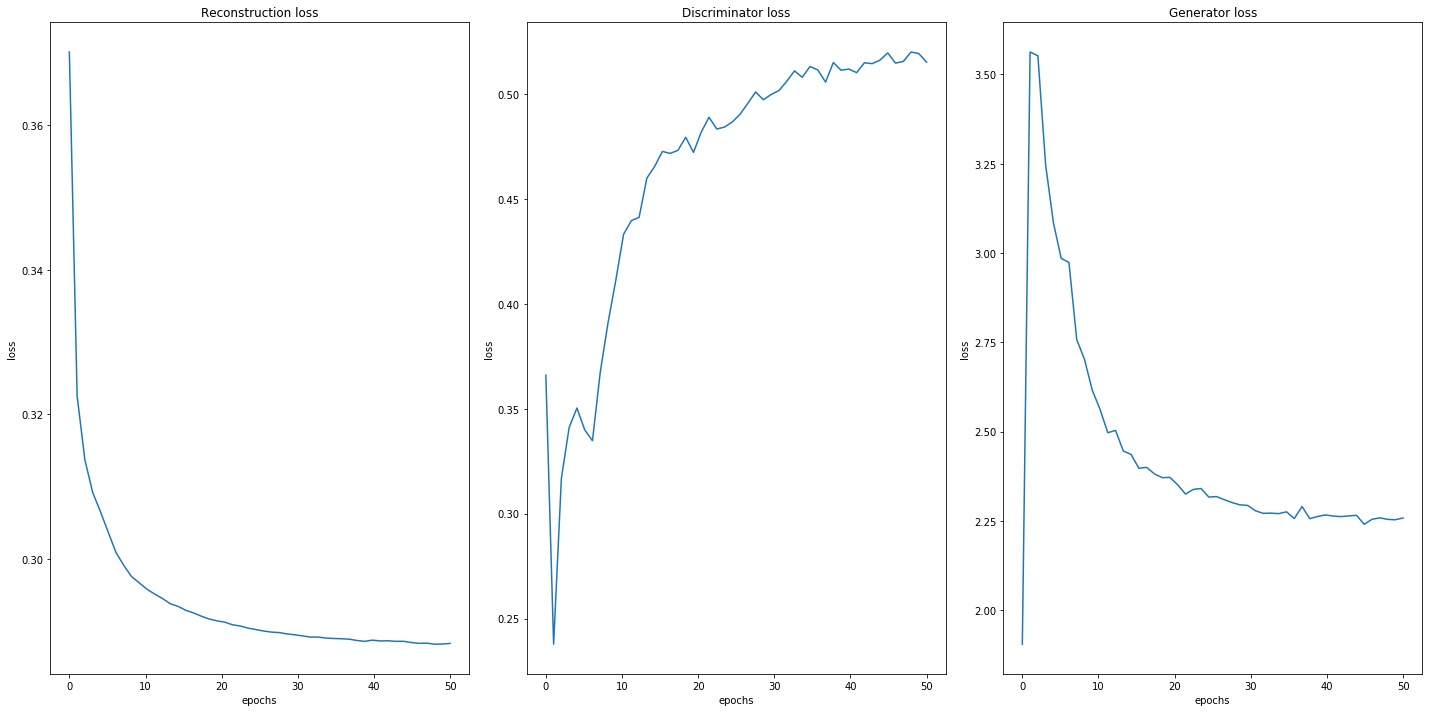
\includegraphics[width=\textwidth]{fashion_plots.png}
\caption{\label{fig:fplot} Training Losses - FashionMNIST}
\end{figure}

\begin{figure}
\centering
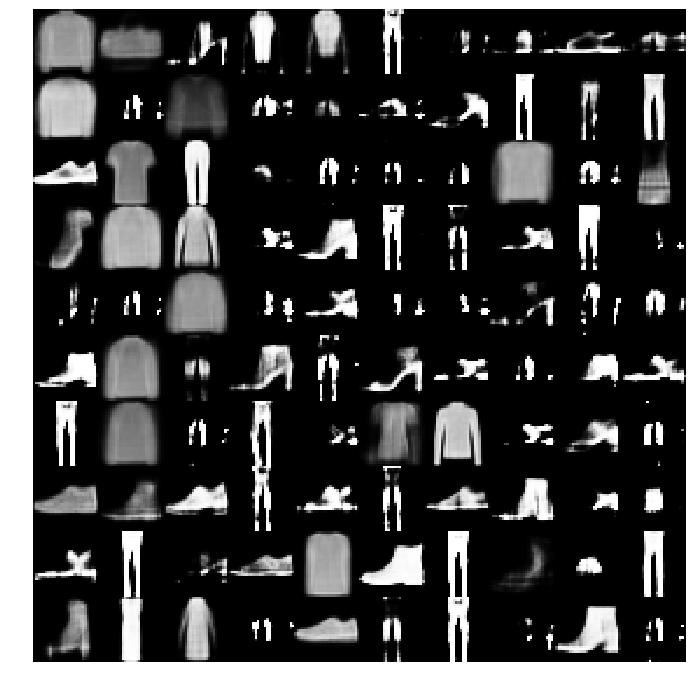
\includegraphics[width=\textwidth]{fashion.png}
\caption{\label{fig:fashion} Generated Images - FashionMNIST}
\end{figure}

\end{document}
